\section{Simulation}
The simulation used the linear-regression detection model, based on the results of the signal detection experiment, together with data on human saccade distributions taken from previous work, to construct a stochastic model of saccade paths during visual search.

\subsection{Human Saccade Distributions}

In this section we will present a new analysis of data from the first of Clarke et al.'s [\citeyear{clarke2009}] visual search experiments. This experiment involved similar stimuli to those described above, although only 3 different target eccentricities were used. Seven observers completed the experiment and the task was simply to press a button on the keyboard once the target had been found. They were given unlimited time and an eye-tracker was used to monitor fixation locations. As the surface was made rougher (decreasing $\beta$ and increasing $\sigma_{RMS}$) a greater number of saccades were required to find the target. We will now carry out some further analysis of this data set. 

\par

The global saccade amplitude and direction distributions are shown in Figure \ref{fig:SaccadeStatistics} (top left and top right). As we can see, the saccade directions show the same horizontal bias as reported by \cite{gilchrist-harvey2006} and \cite{najemnik-geisler2008}. The saccade amplitude time series (Figure \ref{fig:SaccadeStatistics} (bottom left)) shows evidence for a coarse-to-fine search strategy, as reported by \cite{over2007}. 
\par
Figure \ref{fig:spatialsaccadestats} shows the distributions of saccade amplitude and directions according to the location of the starting fixation, in relation to the stimuli boundaries. For example, the largest saccade amplitudes appear to occur after a fixation is made near the corner of the stimuli early on in the search. Again, this agrees with the coarse-to-fine strategy described by Over et al. 
 

\begin{figure}
	\centering
		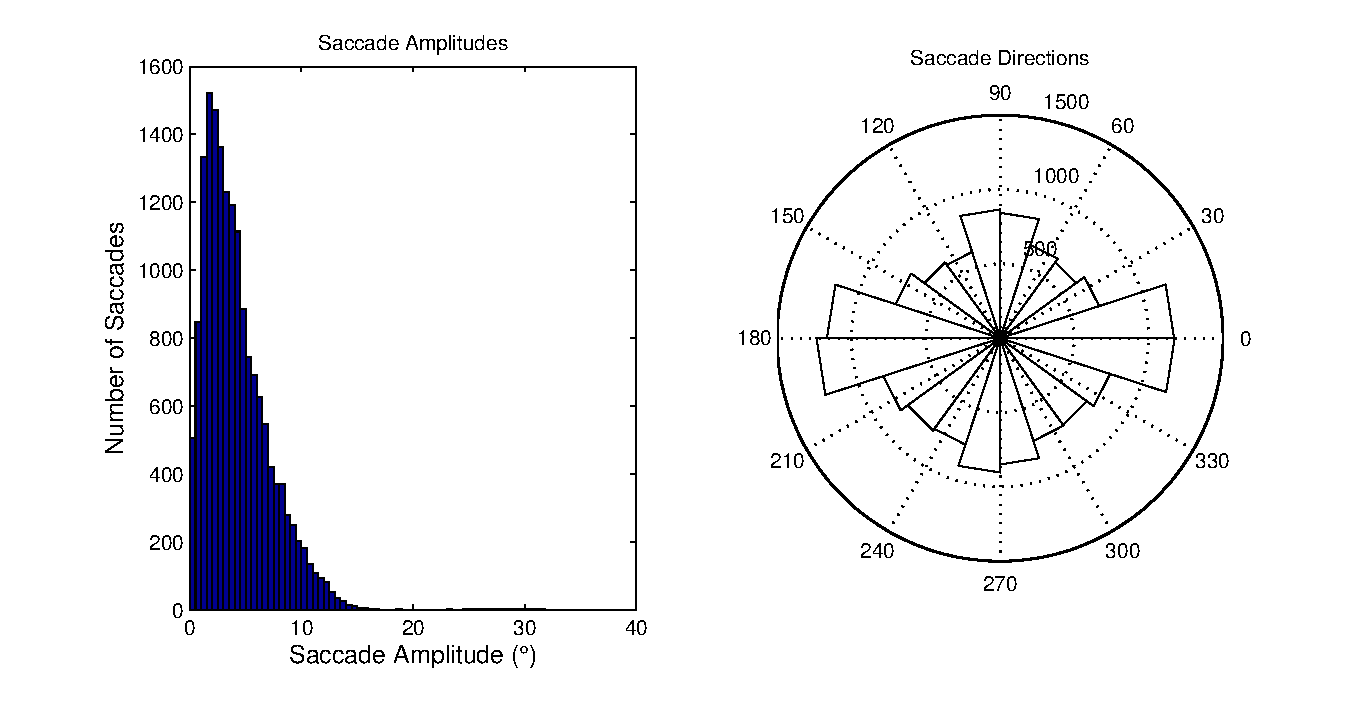
\includegraphics[width=7.5cm]{figures/SaccadeHistandRose.eps}
			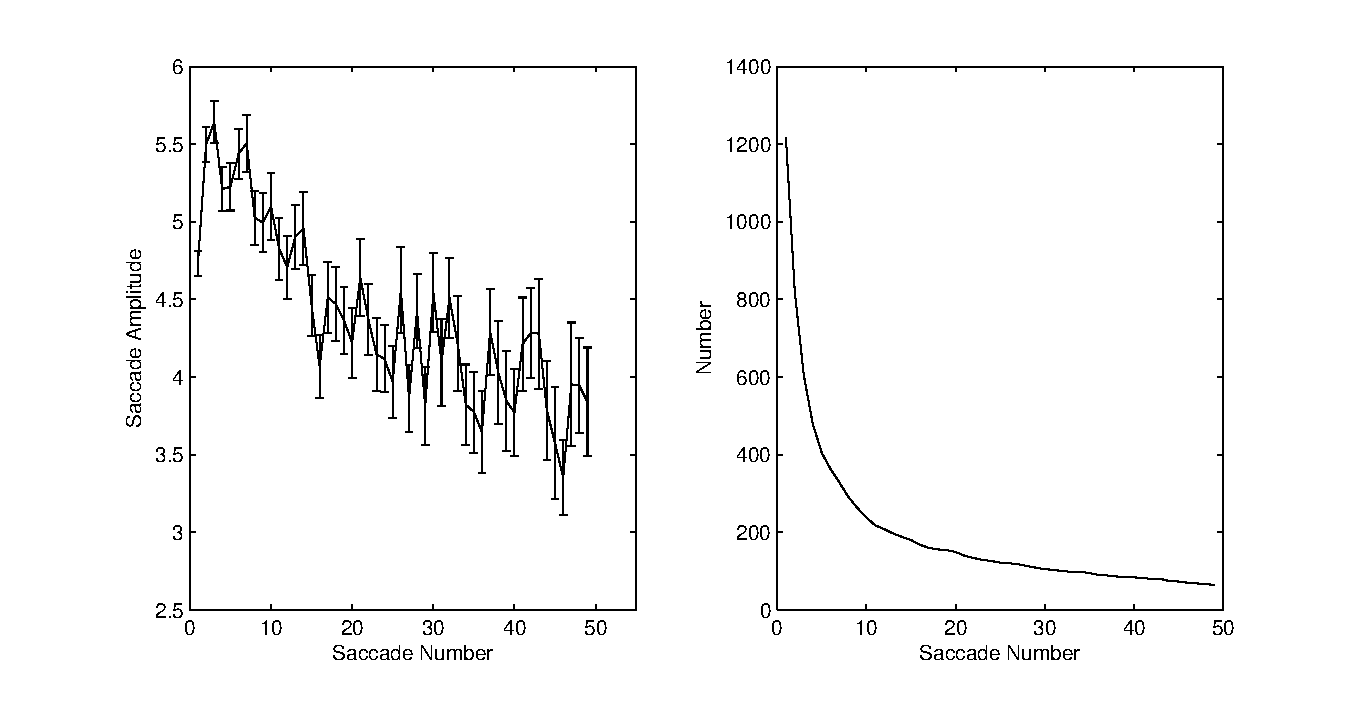
\includegraphics[width=7.5cm]{figures/SaccadeAmpOverTime.eps}
	\caption{(Top Left) Saccade amplitude histogram, (Top Right) Saccade direction rose plot, (Bottom Left) Saccade amplitude plotted against time, and (Bottom Right) The number of the fixations included in the analysis on the left.}
	\label{fig:SaccadeStatistics}
\end{figure}


\subsection{Algorithm}

\subsubsection{Inputs}
The model is given the size of the search area, $N$, the roughness of the surface $\beta$, and the target location (chosen randomly for a given eccentricity $r$). The initial fixation is set to the centre of the search area.

\subsubsection{Target Detection}
On each fixation the probability that the model detects the target is given by $p=f(\beta,r)$ where $f$ is the linear regression model described above. For each fixation we generate a random number $x\in[0,1]$ and check to see if $x\leq p$, in which case the model detects the target, makes a saccade to the target's location, and the search is terminated. If the model does not detect the target (i.e. $x>p$) then a random saccade is made to a new location. 

\subsubsection{Generating a Saccade}
In order to generate scan-paths we will use the empirical distributions of saccades (Figure \ref{fig:spatialsaccadestats}) as probability density functions. Since the amplitude distribution varies with the position of a saccade in the sequence made during a search trial we use separate empirical distributions for fixations $1\leq t\leq 5$, $6\leq t\leq 10$, $11\leq t \leq 15$ and $t>15$ (where $t$ is the fixation number). %The model is allowed to make a maximum of 200 fixations.

\begin{figure*}
	\centering
		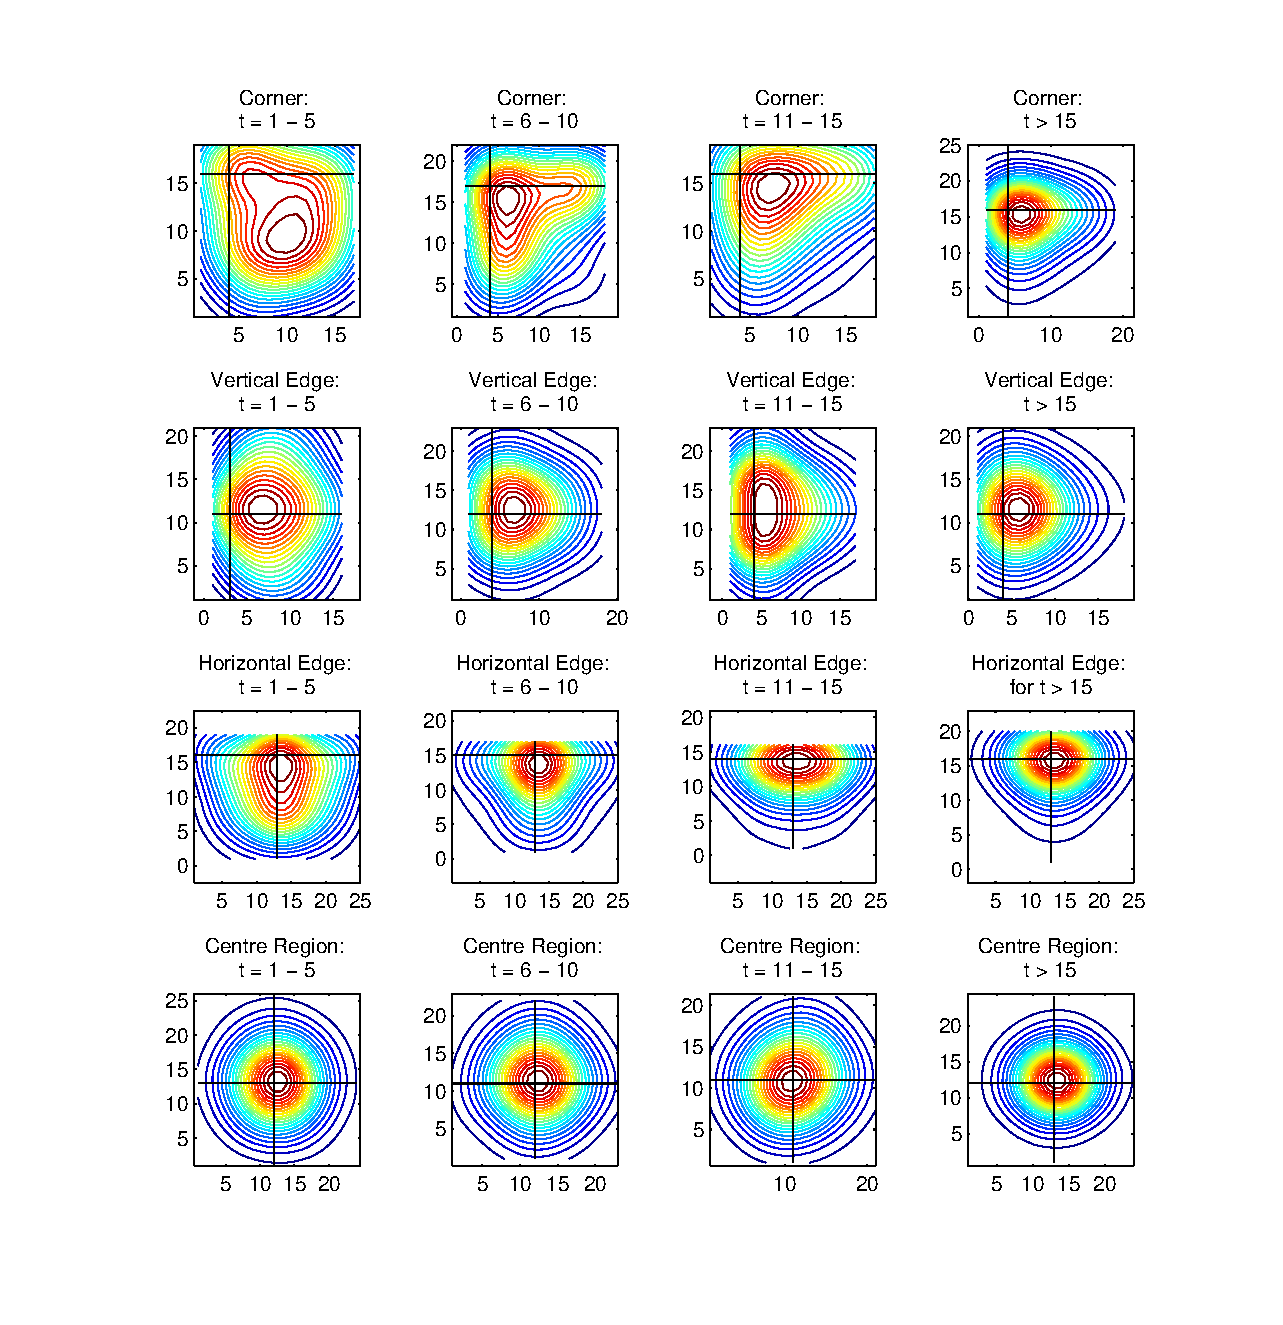
\includegraphics[width=14cm]{figures/saccadesbyposition2.eps}
		\caption{The effect of time and fixation location on saccades. These were created by dividing the search area into $5\times 5$ equally sized subregions. Horizontal and vertical axis of symmetry were assumed and used to combine information from the four corners regions. Similarly, the three remaining subregions along the left edge were reflected and combined with those along the right edge (similar for the top and bottom edges). Finally the nine central regions were grouped together.}
	\label{fig:spatialsaccadestats}
\end{figure*}


\subsubsection{Results}
Considering first the performance of the model in terms of the number of fixations required to find the target, we see that it performs in a similar way to the human observers in \cite{clarke2009} (Figure \ref{fig:Model_Human_numfix}). While the model slightly overestimates the number of saccades needed on easy surfaces, and underestimates the amount needed for harder surfaces, it remains within the 95\% confidence interval of the mean human observer.  

\par

\begin{figure}
	\centering		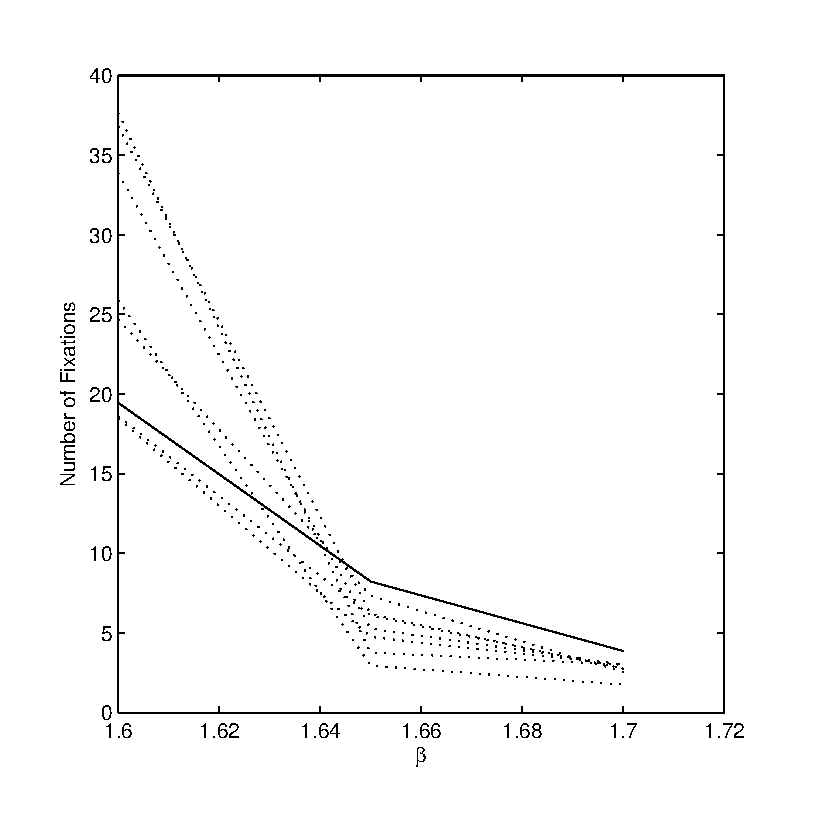
\includegraphics[width=7.5cm]{figures/Model_Human_numfix.eps}
		\caption{Comparison between human observers and the model. The top graph shows the performance, in terms of the number of fixations required to find the target, for each of the seven participants (dashed line), while the solid line shows the model's performance.}
	\label{fig:Model_Human_numfix}
\end{figure}
Next we compare how efficiently human observers and the model cover the search area during search. If human search has systematic properties we would expect the fixation locations to be approximately uniformly distributed: as there are no salient regions in the image apart from the target there is no reason to fixate any one area more than any other (except for a potential innate central fixation bias \citep{tatler2007}). The hotspot maps for the model and human observers are shown in Figure \ref{fig:hotspot}. For the human data, these included the first 30 fixations (excluding the initial fixation) from all trials in which at least 32 fixations were made (to minimise the effect of detecting the target. The model data was generated by simply running the model 105 times without the target detection component. The two hotspot maps were normalised. As we can see, the model appears to exhibit more of a central bias than the human data.

\begin{figure*}
	\centering
		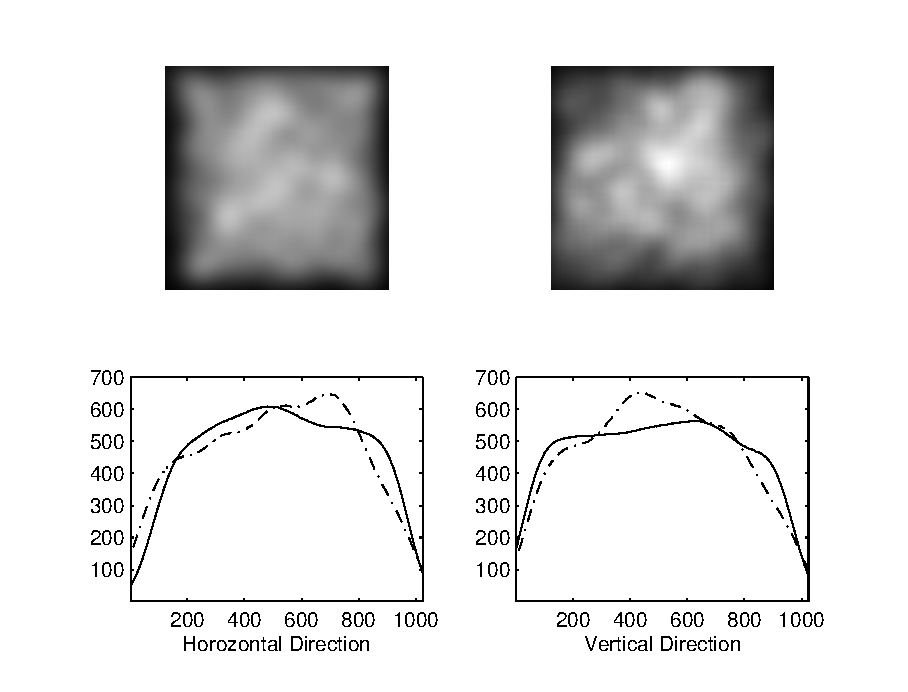
\includegraphics[width=14.9cm]{figures/hotspotcomparison.eps}
	\caption{(top left) Hotspot map of first 30 fixations over all trials (containing over 32 fixations) and observers. (top right) Hotspot map generated by the stochastic model. The stochastic model appears to be more biased towards the centre of the image. (bottom left/right) Density of fixations along the horizontal/vertical directions. Legend: (solid line) human observers (dashed line) stochastic model.}
	\label{fig:hotspot}
\end{figure*}

\par

Another way to compare how systematic human observers are is to look at the number of re-fixations. We have done this by checking each fixation to see if it is located within $30$pixels ($1/2^{\circ}$ of visual angle) of any of the previous three fixations. For each trial we computed the number of refixations per fixation. This number gives us an indication of how strong inhibition of return (IoR) is in the search task considered here and the results (see Figure \ref{fig:refixations}) show that humans appear to be no more systematic than the stochastic simulation. In fact, the model actually makes less re-fixations per fixation on the harder trials.

\begin{figure}
	\centering
		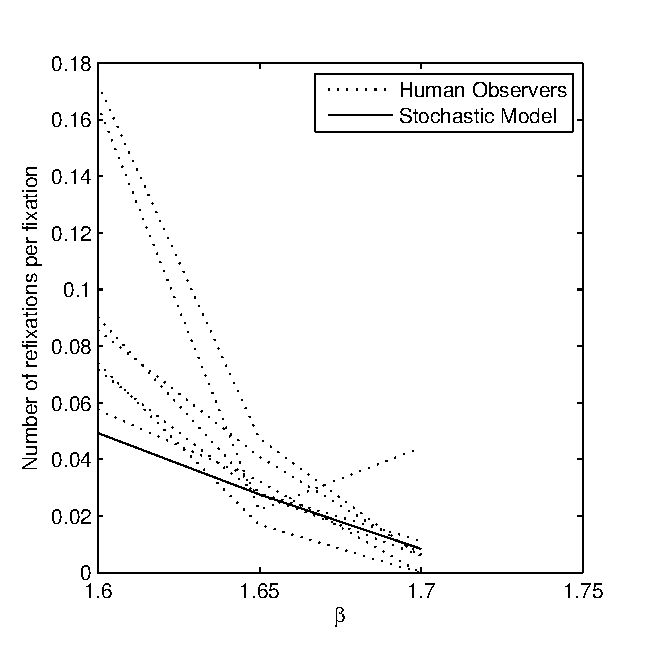
\includegraphics[width=7.5cm]{figures/refixations.eps}
	\caption{Number of times a saccade is directed to the location of one of the previous three fixations, divided by total number of fixations for that trial.}
	\label{fig:refixations}
\end{figure}

\par

Finally, we will use the Voronoi method proposed by \cite{over2006} to compare the distribution of saccades from the human and model. This method allows us to study the uniformity of fixation density and involves computing the bounded Voronoi cells \citep{voronoi1907} for a set of fixation coordinates and looking at the distribution of cell areas. Some examples of Voronoi diagrams can be seen in Figure \ref{fig:VoronoiExamples}. However, instead of looking at the skewness and fitting curves to the distribution of cell areas as Over et al. did, we will look at how the cells change over time, as successive fixations are made. A simple way of doing this is to look at how the area of the largest cell changes with fixation number. If search is systematic then we would expect observers to direct fixations towards regions of the display area which they have not already attended to and the size of the largest cell will fall more steeply than for a stochastic search.
\par

\begin{figure*}
	\centering
	\subfigure[Human Observer]{
		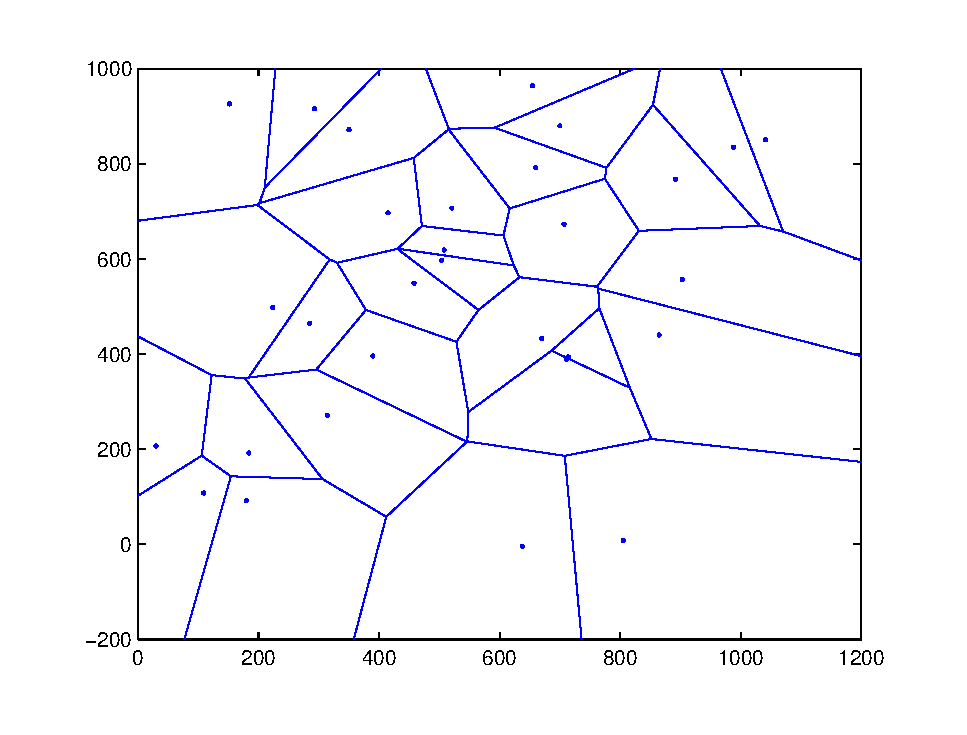
\includegraphics[width=7cm]{figures/Voronoi_new_human1.eps}}
		\subfigure[Human Observer]{
		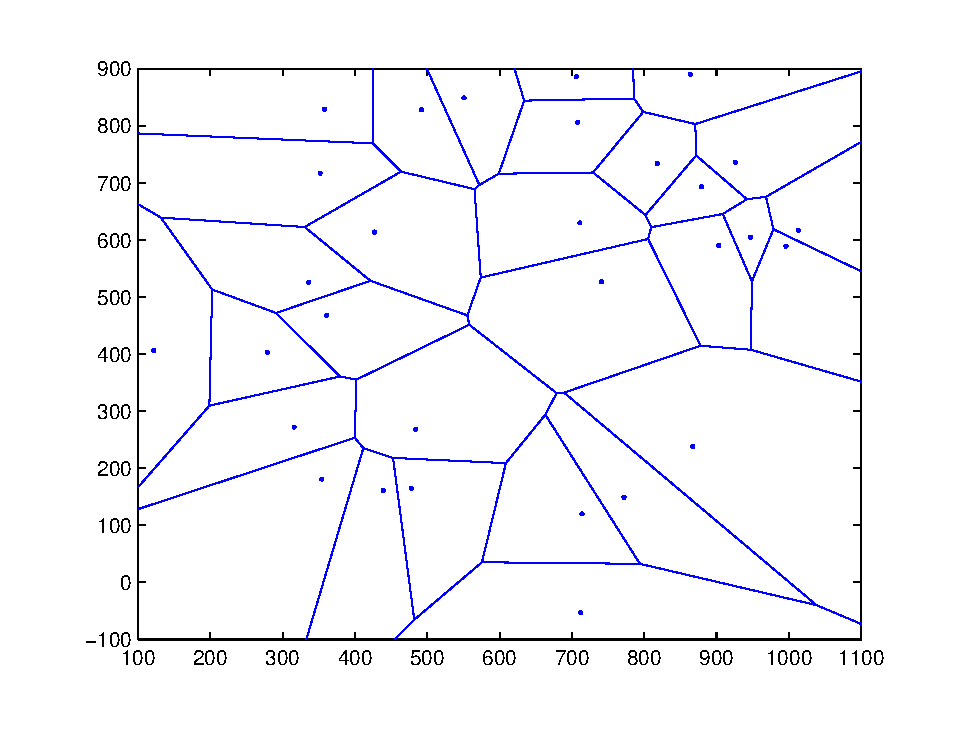
\includegraphics[width=7cm]{figures/Voronoi_new_human2.eps}}
			\subfigure[Model ]{
		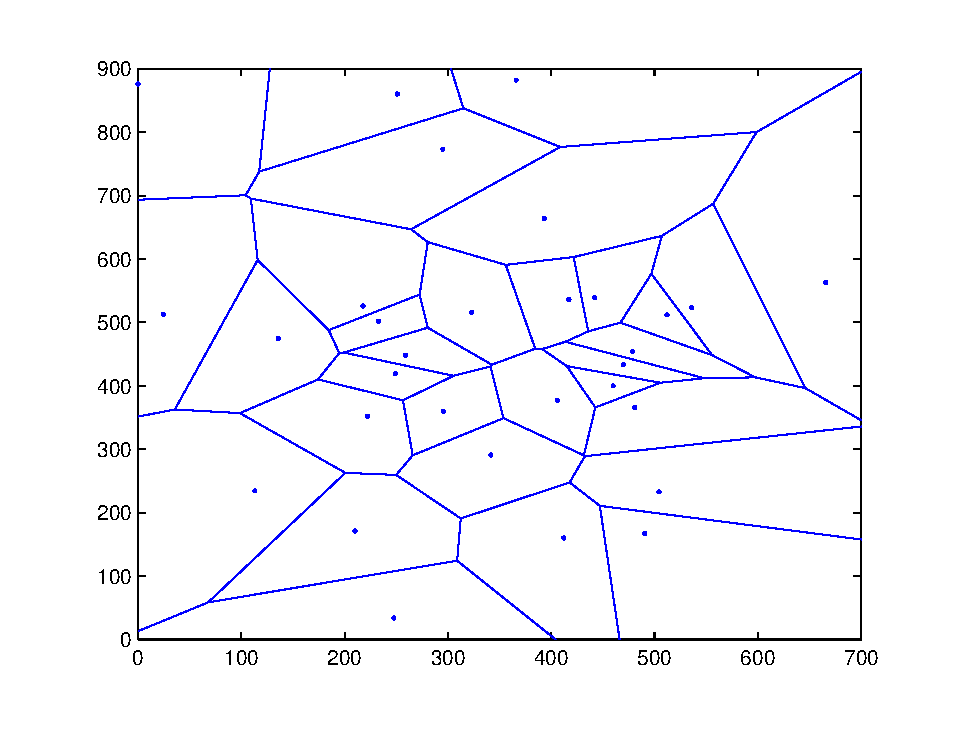
\includegraphics[width=7cm]{figures/Voronoi_new_model1.eps}}
		\subfigure[Model]{
		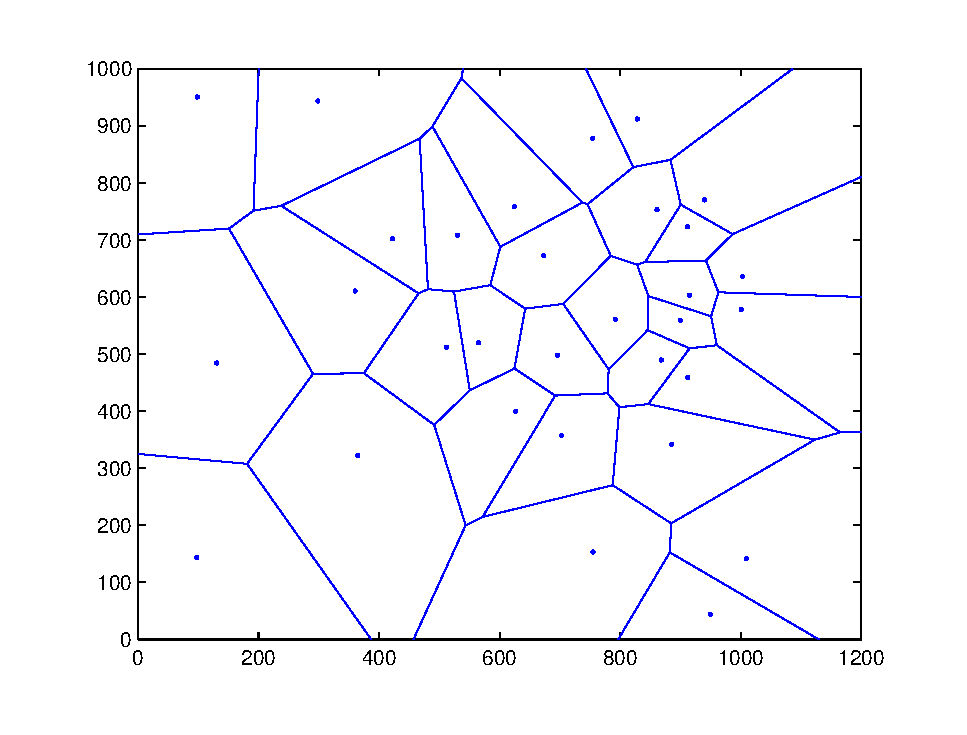
\includegraphics[width=7cm]{figures/Voronoi_new_model2.eps}}
		\caption{Examples of Voronoi plots from both the human observers and the stochastic model.}
	\label{fig:VoronoiExamples}
\end{figure*}


For each fixation $f_t$, ($t=1,\ldots,n-2$, where $n$ is the number of fixations in the trial), the Voronoi cells for fixations $f_1,\ldots,f_t$, are created and the the area of the largest cell, $A_t$ , is computed. The mean $A_t$, over all trials, is shown in Figure \ref{fig:VoronoiTime} (left). As we can see, the human observers outperform the stochastic simulation and the size of the largest Voronoi cell decreases rapidly durng the first 5 fixations. However if we look at the speed at which the observers reduce the size of the cell ($A_t-A_{t+1}$) we see that after the initial five fixations the stochastic simulation matches human performance (Figure \ref{fig:VoronoiTime} (right)).

\par

\begin{figure*}
	\centering
		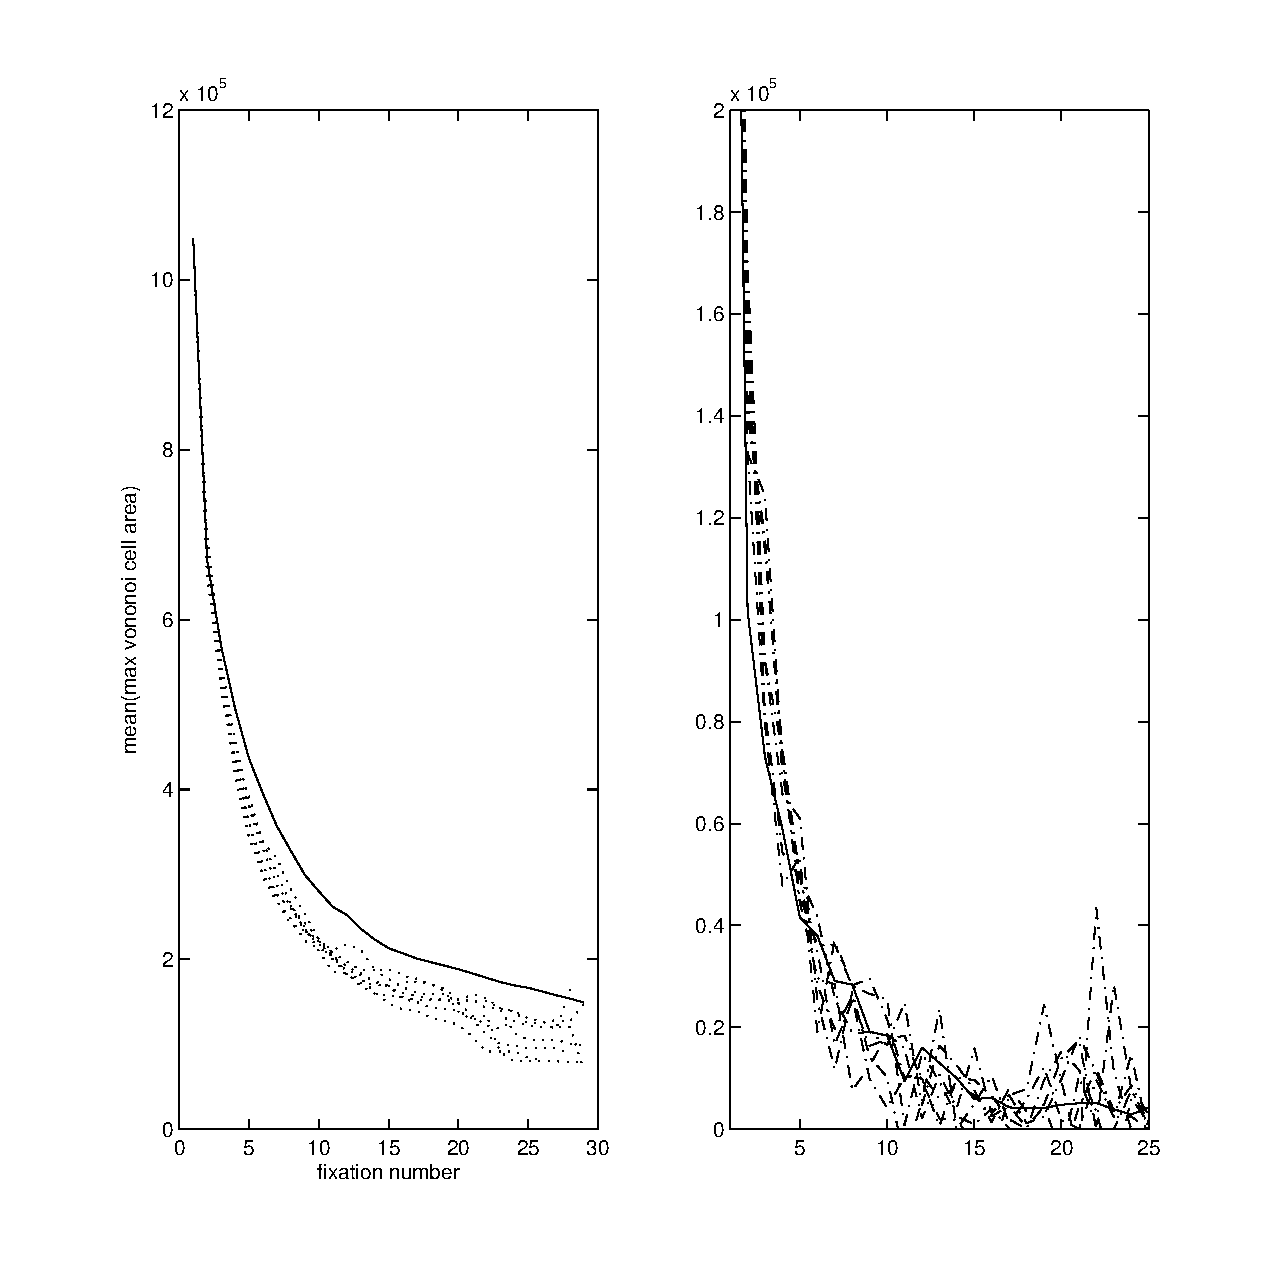
\includegraphics[width=14cm]{figures/VoronoiTime.eps}
	\caption{(left) How the maximum Voronoi cell area changes with time. Dotted lines show the seven human observers while the solid line shows the stochastic model. (right) This shows the derivative of the graph on the left: a measure of how quickly the search area is covered.	he main difference between the model and human observers occurs in the first few fixations. After these inital fixations human observers appear to be no more systematic than the model.}
	\label{fig:VoronoiTime}
\end{figure*}
